\documentclass[a4paper,12pt]{article}

\usepackage[utf8]{inputenc}
\usepackage[left=0.5in,right=0.5in,top=1in,bottom=1in]{geometry}
\usepackage{amsmath,amssymb,amsfonts}
\usepackage{pgfplots,graphicx,calc,changepage}
\pgfplotsset{compat=newest}
\usepackage{enumitem}
\usepackage{fancyhdr}
\usepackage[colorlinks = true, linkcolor = blue]{hyperref}

\newcommand{\nats}{\mathbb{N}}
\newcommand{\reals}{\mathbb{R}}
\newcommand{\rats}{\mathbb{Q}}
\newcommand{\ints}{\mathbb{Z}}
\newcommand{\pols}{\mathcal{P}}
\newcommand{\cants}{\Delta\!\!\!\!\Delta}
\newcommand{\eps}{\varepsilon}
\newcommand{\st}{\backepsilon}
\newcommand{\abs}[1]{\left| #1 \right|}
\newcommand{\dom}[1]{\mathrm{dom}\left(#1\right)}
\newcommand{\for}{\text{ for }}
\newcommand{\dd}[1]{\mathrm{d}#1}
\newcommand{\spn}{\mathrm{sp}}
\newcommand{\nul}{\mathcal{N}}
\newcommand{\col}{\mathrm{col}}
\newcommand{\rank}{\mathrm{rank}}
 \newcommand{\sech}{\mathrm{sech}}
\newcommand{\norm}[1]{\lVert #1 \rVert}
\newcommand{\inner}[1]{\left\langle #1 \right\rangle}
\newcommand{\pmat}[1]{\begin{pmatrix} #1 \end{pmatrix}}
\renewcommand{\and}{\text{ and }}

\newsavebox{\qed}
\newenvironment{proof}[2][$\square$]
    {\setlength{\parskip}{0pt}\par\textit{Proof:} #2\setlength{\parskip}{0.25cm}
        \savebox{\qed}{#1}
        \begin{adjustwidth}{\widthof{Proof:}}{}
    }
    {
        \hfill\usebox{\qed}\end{adjustwidth}
    }

\pagestyle{fancy}
\fancyhead{}
\lhead{Caleb Jacobs}
\chead{APPM 5480: Asymptotics}
\rhead{Homework \#1}
\cfoot{}
\setlength{\headheight}{35pt}
\setlength{\parskip}{0.25cm}
\setlength{\parindent}{0pt}

\begin{document}
\begin{enumerate}[label = \arabic*)]
    \item Find two-term asymptotic approximations to each of the roots of
    \begin{enumerate}[label = (\alph*)]
        \item $ \eps x^3 + \eps x^2 - x + 1 = 0 $.

        First, let's find the regularly perturbed solutions by assuming
        \[
            x = x_0 + \eps x_1 + \eps^2 x_2 + \cdots.
        \]
        Then, our equation becomes
        \[
            \eps(x_0 + \eps x_1 + \eps^2 x_2 + \cdots)^3 + 
            \eps(x_0 + \eps x_1 + \eps^2 x_2 + \cdots)^2 - 
            (x_0 + \eps x_1 + \eps^2 x_2 + \cdots) + 1 = 0.
        \]
        So, equating our ordered terms, we have
        \[
        	\begin{array}{rccl}
            	O(1): & - x_0 + 1 = 0 & \implies & x_0 = 1 \\
            	O(\eps): & x_0^3 + x_0^2 - x_1 = 0 & \implies & x_1 = 2.
        	\end{array}
       \] 
        So, our regularly perturbed root has a two-approximation of
        \[
            \boxed{x = 1 + 2\eps + O(\eps^2).}
        \]
        Now to get our singularly perturbed solutions, suppose
        \[
        	x = \frac{1}{\sqrt{\eps}} y,
        \]
        Then, our equation becomes
        \[
        	\frac{1}{\sqrt{\eps}} y^3 + y^2 - \frac{1}{\sqrt{\eps}} y + 1 = 0 \implies y^3 + \sqrt{\eps} y^2 - y + \sqrt{\eps} = 0
        \]
        which is maximally balanced. Now, assume we can express $ y $ as 
        \[
        	y = y_0 + \sqrt{\eps} y_1 + \cdots.
        \]
        Then, equating our ordered terms yields
        \[
        	\begin{array}{rccl}
        		O(1): &  y_0^3 - y_0 = 0 & \implies & y_0 = -1, 0, 1 \\
        		O(\sqrt{\eps}): & 3y_0^2 y_1 + y_0^2 - y_1 + 1 = 0 & \implies & y_1 = 
        		\begin{cases}
        			-1, & y_0 = \pm 1 \\
        			1, & y_0 = 0
        		\end{cases}.
        	\end{array}
        \]
        We can ignore the case when $ y_0 = 0 $ because that will just lead to our regularly perturbed solution. So our singularly perturbed solutions are given by
        \[
        	\boxed{\begin{array}{l}
        		x = \frac{1}{\sqrt{\eps}} - 1 + O(\sqrt{\eps}) \\
        		x = -\frac{1}{\sqrt{\eps}} - 1 + O(\sqrt{\eps}).
        	\end{array}}
        \]
        The order of accuracy can be found at the end of each expression in the Big-O notation. Furthermore, a convergence plot for this part can be found at the end of the problem.
        
        \newpage
        \item $ 2 \eps^3 x^5 - \eps x^4 + x^3 - 3 \eps x^2 + 4x + 2 \eps = 0 $.
        
        Just like last time, let's find the regularly perturbed solutions by assuming
        \[
        	x = x_0 + \eps x_1 + \eps^2 x_2 + \eps^3 x_3\cdots.
        \]
        Then, plugging in our series for $ x $ into the polynomial equation and equating ordered terms yields
        \[
        	\begin{array}{rccl}
        		O(1): & x_0^3 + 4x_0 = 0 & \implies & x_0 = -2i, 0, 2i \\
        		O(\eps): & -x_0^4 + 3x_0^2x_1 - 3x_0^2 + 4x_1 + 2 = 0 & \implies & x_1 = 
        		\begin{cases}
        			-\frac{1}{4}, & x_0 = \pm 2i \\
        			-\frac{1}{2}, & x_0 = 0
        		\end{cases}.
        	\end{array}
        \]
        We still need one more nonzero term for the case when $ x_0 = 0 $. So when $ x_0 = 0 $, we have
        \[
        	\begin{array}{rccl}
        		O(\eps^2): & 4x_2 = 0 & \implies & x_2 = 0 \\
        		O(\eps^3): & x_1^3 -3 x_1^2 + 4 x_3 = 0 & \implies & x_3 = \frac{7}{32}.
        	\end{array}
        \]
        So, our three regularly perturbed solutions have the form
        \[
	        \boxed{\begin{array}{l}
	        	x = -2i - \frac{1}{4} \eps + O(\eps^2), \\
	        	x = -\frac{1}{2} \eps + \frac{7}{32} \eps^3 + O(\eps^5), \\
	        	x = 2i -  \frac{1}{4} \eps + O(\eps^2).
	        \end{array}}
    	\]
    	
    	Now, let's look for singularly perturbed solutions by first considering
    	\[
    		x = \frac{1}{\eps^2} y.
    	\]
    	In this case, our equation becomes
    	\[
    		2 y^5 - y^4 + \eps y^3 - 3 \eps^4 y^2 + 4 \eps^4 y + 4 \eps^5 y + 2 \eps^8 = 0
    	\]
    	which is maximally balanced by the first two terms. Just as before,
    	let's assume
    	\[
    		y = y_0 + \eps y_1 + \eps^2 y_2 + \cdots.
    	\]
    	Now, plugging this in and equating our ordered terms yields
    	\[
    			O(1): 2y_0^5 - y_0^4 = 0 \implies y_0 = 0, \frac{1}{2}.
    	\]
    	Now, just taking $ y_0 = \frac{1}{2} $, we have
    	\[
    		O(\eps): 10y_0^4 - 4y_0^3y_1 + y_0^3 = 0 \implies  y_1 = -1
    	\]
    	which gives a solution of 
    	\[
    		\boxed{x = \frac{1}{2\eps^2} - \frac{1}{\eps} + O(1).}
    	\]
    	To find the other singularly perturbed solutions, assume
    	\[
    		x = \frac{1}{\eps} y.
    	\]
    	Then, our equation becomes
    	\[
    		2 \eps y^5 - y^4 + y^3 - 3\eps^2 y^2 + 4 \eps^2 y + 2 \eps^4 = 0
    	\]
    	which implies
    	\[
    		O(1): -y_0^4 + y_0^3 = 0 \implies y_0 = 0, 1.
    	\]
    	Then, taking $ y_0 = 1 $ yields
    	\[
    		O(\eps): 2 - 4y_1 + 3y_1 = 0 \implies y_1 = 2.
    	\]
    	So, our final singularly perturbed solution is given by
    	\[
    		\boxed{x = \frac{1}{\eps} + 2 + O(\eps).}
    	\]
    	
    	Just like part (a), the order of accuracy for each approximation is in Big-O notation at the end of the estimate. To confirm the order of accuracies, the plot below shows the convergence of each root estimate.
    	
    	\newpage
    	\begin{figure}[h!]
    		\centering
    		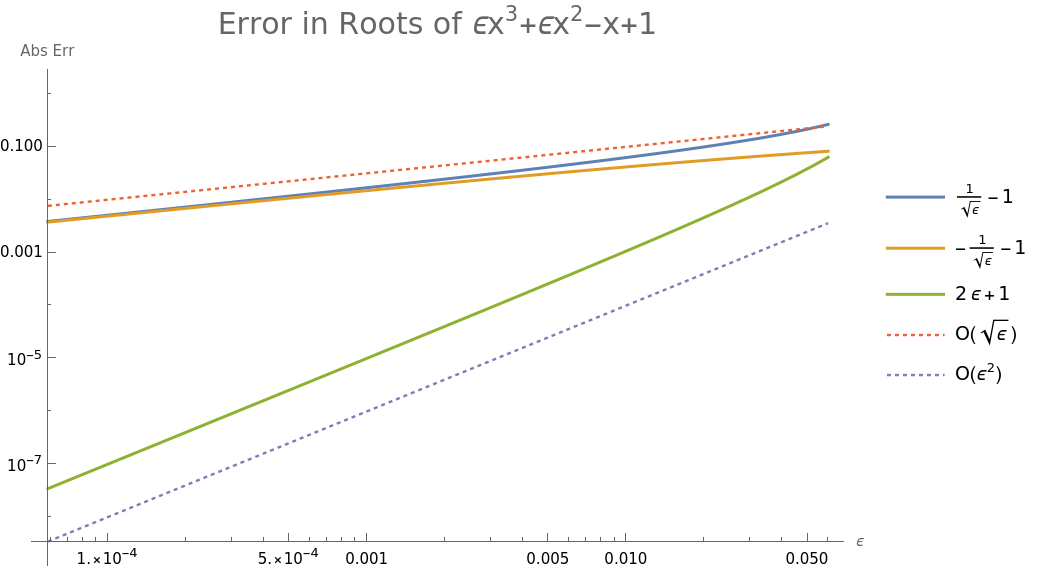
\includegraphics[width = 0.9\textwidth]{Images/1a.png}
    	\end{figure}
    
    	\vspace{3cm}
    	
    	\begin{figure}[h!]
    		\centering
    		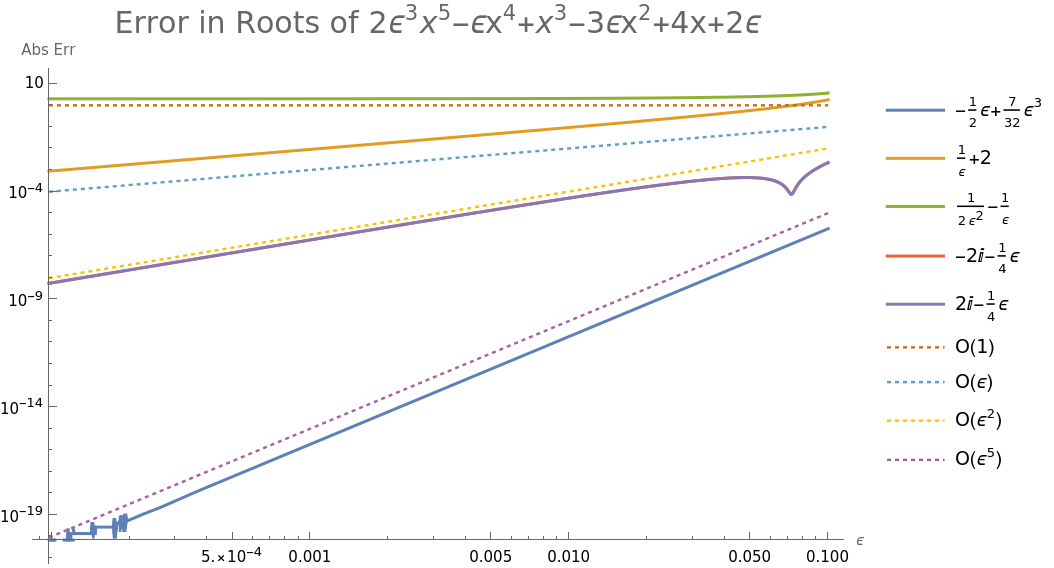
\includegraphics[width = 0.9\textwidth]{Images/1b.png}
    	\end{figure}
    \end{enumerate}
	
	\newpage
	\item Find the first three terms of an asymptotic approximation to the solution $ x(\eps) $ of the transcendental equation
	\[
		\frac{e^{-x^2}}{x} = \eps, \quad \eps \ll 1.
	\]
	
	To find our approximation, we will use an iterative method. The iteration can be set up as follows
	\begin{align*}
		& e^{-x^2} = \eps x \\
		\implies & -x^2 = \ln(\eps) + \ln(x) \\
		\implies & x^2 = \ln\left(\frac{1}{\eps}\right) - \ln(x)
	\end{align*}
	which gives us the iteration scheme
	\[
		x_n^2 = \ln\frac{1}{\eps} - \ln x_{n-1}
	\]
	Now, suppose $ x_0 = 1 $. Then if we let $ L_1 = \ln\frac{1}{\eps} $, iterating yields
	\[
		x_1^2 = \ln\frac{1}{\eps} = L_1.
	\]
	Next, let $ L_2 = -\frac{1}{2} \ln\ln\frac{1}{\eps} = -\frac{1}{2} \ln L_1 $. Then iterating again
	\[
		x_2^2 = \ln\frac{1}{\eps} - \ln\sqrt{\ln\frac{1}{\eps}} = \ln\frac{1}{\eps} - \frac{1}{2} \ln\ln\frac{1}{\eps} = L_1 + L_2.
	\]
	Again,
	\begin{align*}
		x_3^2 &= L_1 - \ln (L_1 + L_2) \\
		&= L_1 - \frac{1}{2} \ln \left(L_1\left(1 + \frac{L_2}{L_1}\right)\right) \\
		&= L_1 + L_2 - \frac{1}{2} \ln\left(1 + \frac{L_2}{L_1}\right) \\
		&= L_1 + L_2 - \frac{1}{2} \frac{L_2}{L_1} + \frac{1}{4} \left(\frac{L_2}{L_1}\right)^2 + \cdots
	\end{align*}
	So, truncating our series yields the asymptotic approximation
	\[
		\boxed{x^2 \sim L_1 + L_2 - \frac{1}{2} \frac{L_2}{L_1} \text{ as } \eps \to 0.}
	\]
	\newpage
	\item Find the first order perturbations of the eigenvalues of the differential equation
	\[
		\left\{\begin{array}{lc}
			y'' + \lambda y + \eps y^n = 0, & x \in (0, \pi) \\
			y(0) = y(\pi) = 0
		\end{array}\right.
	\]
	for $ n = 1, 2 , 3 $.
	
	First, let's compute the eigenvalues and eigenfunctions for the unperturbed problem:
	\[
		y_0'' + \lambda y_0 = 0 \implies y_0 = A \cos(\sqrt{\lambda} x) + B \sin(\sqrt{\lambda} x).
	\]
	Then, from the BCs,
	\[
		y_0(0) = A = 0
	\]
	and
	\[
		y_0(\pi) = B \sin(\sqrt{\lambda} \pi) = 0 \implies \lambda_0 = k^2, \quad k = 1, 2, \ldots.
	\]
	Next, from the Fredholm alternative, we can compute our first order eigenvalue term as
	\[
		\lambda_1 = \frac{\inner{(y_0)^n, w}}{\inner{y_0, w}}
	\]
	where 
	\[
		(\mathcal{L}^* - \lambda_0^*)w = -w'' - k^2 w = 0
	\]
	which implies
	\[
		w(x) = A \sin(k x).
	\]
	Then,
	\[
		\lambda_1 = \frac{\inner{\sin^n(k x), A\sin(k x)}}{\inner{\sin(k x), A\sin(k x)}} = \frac{\int_{0}^{\pi} A^n \sin^{n + 1}(x) \dd{x}}{\int_{0}^{\pi} A \sin^2(x) \dd{x}} = 
		\begin{cases}
			1, & n = 1 \\
			\frac{4}{3k\pi}A(1 - (-1)^k), & n = 2 \\
			\frac{3 A^2}{4}, & n = 3
		\end{cases}.
	\]
	So, putting everything together, we have the 1st order perturbation for $ \lambda $ as
	\[
		\boxed{\lambda = k^2 +
			\eps \left(\begin{cases}
				1, & n = 1 \\
				\frac{4}{3k\pi}A(1 - (-1)^k), & n = 2 \\
				\frac{3 A^2}{4}, & n = 3
			\end{cases}\right) + O(\eps^2).}
	\]
	I know for odd $ k $, the 1st order term goes to zero when $ n = 2 $ but I can not for the life of me figure out how to get a ``$ \lambda_2 $'' to keep two nonzero terms there.
	
	\newpage
	\item Bessel's function of the first kind and $ 3/2 $ order is given by
	\[
		J_{3/2}(x) = \sqrt{\frac{2}{\pi x}} \left(- \cos x + \frac{\sin x}{x}\right).
	\]
	Determine the two-term expansions for large roots of
	\begin{enumerate}[label = (\alph*)]
		\item $ J_{3/2}(x) = 0 $.
		
		First, note that 
		\begin{align*}
			J_{3/2}(x) = 0 \implies & \sqrt{\frac{2}{\pi x}} \left(- \cos x + \frac{\sin x}{x}\right) = 0 \\
			\implies & - \cos x + \frac{\sin x}{x} = 0 \\
			\implies & \cot(x) = \frac{1}{x}.
		\end{align*}
		From our final expression, when $ \abs{x} \gg 0 $, we would expect $ \cot(x) $ to dominate the solution to the roots because $ \frac{1}{x} $ decays. So we would expect large roots to look like the roots of $ \cot(x) $ plus some corrector. The roots of $ \cot(x) $ are given by
		\[
			x_{\cot} = (2k + 1)\frac{\pi}{2}, \quad k \in \ints.
		\]
		So, let's assume our solution is of the form
		\[
			x = x_{\cot} + \delta(k)
		\]
		where $ \delta(k) $ is our corrector. Then, rewriting our equation and expanding about $ x_{\cot} $ yields
		\begin{align*}
			\cot(x) = \frac{1}{x} \implies & \sin(x) = x \cos(x) \\
			\implies & (-1)^k + O(x^2) = \frac{1}{4} \pi  (-1)^k (2 k+1) (2 \pi  k-2 x+\pi ) + O(x^2)
		\end{align*}
		Then, substituting $ x = x_{\cot} + \delta(k) $ in and truncating yields
		\begin{align*}
			& (-1)^k = -(-1)^k (2k + 1)  \frac{\pi}{2} \delta(k) \\
			\implies & \delta(k) = -\frac{2}{2k\pi + \pi} + O\left(\frac{1}{k^2}\right).
		\end{align*}
		Putting everything together, we have an approximate solution of
		\[
			\boxed{x = x_{\cot} + \delta(k) = (2k + 1)\frac{\pi}{2} - \frac{2}{2k\pi + \pi} + O\left(\frac{1}{k^4}\right).}
		\]
		
		I know the problem asked for a comparison with the first 5 roots but I went a bit further to a 100 roots to see the trend continue; the convergence plot is at the end of the problem.
		
		\item $ J'_{3/2}(x) = 0 $.
		
		Somewhat similar to before, we have
		\begin{align*}
			J'_{3/2}(x) = 0 \implies & \frac{\left(2 x^2-3\right) \sin (x)+3 x \cos (x)}{\sqrt{2 \pi } x^{5/2}} = 0 \\
			\implies & \left(2 x^2-3\right) \sin (x)+3 x \cos (x) = 0 \\
			\implies & \tan(x) = \frac{3x}{3 - 2x^2}.
		\end{align*}
		From this expression, we can see that for large $ x $, the $ \tan(x) $ is the dominant term so we would expect the roots of $ \tan(x) $ to dominate the solution. In this case, we have the roots of $ \tan(x) $ as
		\[
		x_{\tan} = k \pi, \quad k \in \ints.
		\]
		Now, let's assume the roots of our equation have the form
		\[
			x = x_{\tan} + \delta(k)
		\]
		where $ \delta(k) $ is a correction. Then rewriting our equation, expanding about $ x_{\tan} $, and plugging in our assumption yields
		\begin{align*}
			\tan(x) = \frac{3x}{3 - 2x^2} \implies & \left(3 - 2 x^2\right) \sin (x) = 3 x \cos (x) \\
			\implies & (-1)^k \left(3-2 \pi ^2 k^2\right) (x-\pi  k) = 3 (-1)^k x + O(x^2) \\
			\implies & (-1)^k(3 - 2k^2 \pi^2)\delta(k) = 3(-1)^k (k \pi + \delta(k)) \\
			\implies & \delta(k) = -\frac{3}{2 k \pi} + O\left(\frac{1}{k^4}\right).
		\end{align*}
		So, our large roots can be approximated using
		\[
			\boxed{x = x_{\tan} + \delta(k) = k\pi - \frac{3}{2 k \pi}.}
		\]
		The convergence plot can be found on the next page.
		
		\newpage
		\begin{figure}[ht]
			\centering
			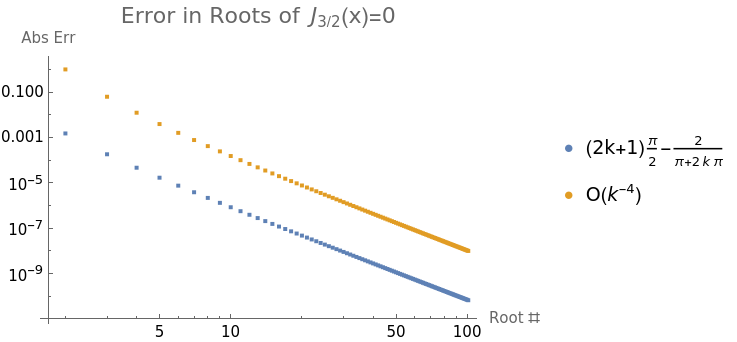
\includegraphics[width = 0.9\textwidth]{Images/4a.png}
		\end{figure}
		
		\begin{figure}[ht]
			\centering
			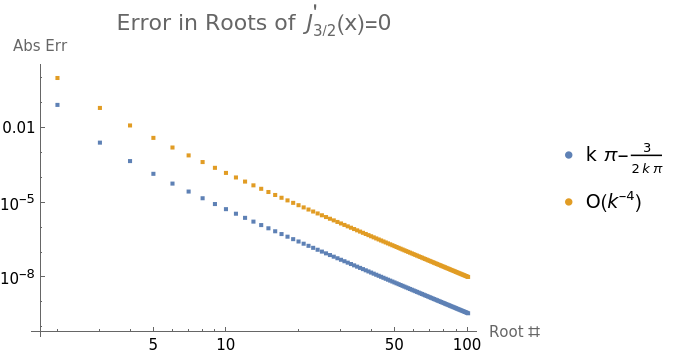
\includegraphics[width = 0.9\textwidth]{Images/4b.png}
		\end{figure}
	\end{enumerate}
	
	\newpage
	\item Determine the order of the following as $ \eps \to 0 $:
	\begin{enumerate}[label = (\alph*)]
		\item $ \ln(\cot \eps) $
		\[
			\ln(\cot \eps) = \ln \left(\frac{\cos \eps}{\sin \eps}\right) = \ln\left(\frac{1 - \frac{1}{2}\eps^2 + \cdots}{\eps - \frac{1}{6} \eps^3 + \cdots}\right) \sim \ln\left(\frac{1}{\eps}\right) = O\left(\ln\left(\frac{1}{\eps}\right)\right)
		\]
		
		\item $ \sinh \frac{1}{\eps} $
		\[
			\sinh \frac{1}{\eps} = \frac{1}{2} (e^{\frac{1}{\eps}} - e^{-\frac{1}{\eps}}) \sim \frac{1}{2}e^{\frac{1}{\eps}} = O(e^{\frac{1}{\eps}})
		\]
		
		\item $ \coth \frac{1}{\eps} $
		\[
			\coth \frac{1}{\eps} = \frac{e^{\frac{1}{\eps}} + e^{-\frac{1}{\eps}}}{e^{\frac{1}{\eps}} - e^{-\frac{1}{\eps}}} \sim \frac{e^{\frac{1}{\eps}}}{e^{\frac{1}{\eps}}} = 1 = O(1)
		\]
		
		\item $ \frac{\eps^{3/4}}{1 - \cos \eps} $
		\[
			\frac{\eps^{3/4}}{1 - \cos \eps} = \frac{\eps^{3/4}}{1 - 1 + \frac{1}{2}\eps^2 + \cdots} = \frac{\eps^{3/4}}{\frac{1}{2}\eps^2 + \cdots} \sim 2\eps^{3/4 - 2} = 2\eps^{-5/4} = O(\eps^{-5/4})
		\]
		
		\item $ \ln \left(1 + \ln \frac{1 + 2 \eps}{\eps}\right) $
		\[
			\ln \left(1 + \ln \frac{1 + 2 \eps}{\eps}\right) = \ln \left(1 + \ln \left(\frac{1}{\eps} + 2 \right)\right) \sim \ln \left(1 + \ln \frac{1}{\eps}\right) = O\left(\ln \left(\ln \frac{1}{\eps}\right)\right)
		\]
	\end{enumerate}

	\item Arrange the following in descending order for small $ \eps $
	\begin{enumerate}[label = (\alph*)]
		\item Given $ e^{-1/\eps}, \ln \frac{1}{\eps}, \eps^{-0.01}, \cot \eps, \sinh \frac{1}{\eps} $, we can order them in descending order as
		\[
			\sinh \frac{1}{\eps} \gg \cot \eps \gg \eps^{-0.01} \gg \ln \frac{1}{\eps} \gg e^{-1/\eps}.
		\]
		This ordering was pretty straight forward although $ \eps^{-0.01} $ and $ \ln \frac{1}{\eps} $ was a little tricky until I noticed the limit of the ratio between the two went to zero when $ \ln \frac{1}{\eps} $ was in the numerator.
		
		\item Given $ \ln(1 + \eps) = O(\eps), \cot \eps = O\left(\frac{1}{\eps}\right), \tanh \frac{1}{\eps} = O(1), \frac{\sin \eps}{\eps^{3/4}} = O(\eps^{1/4}), \eps \ln \eps, e^{-1/\eps}, \sinh \frac{1}{\eps} = O(e^{1/\eps}), \frac{1}{\ln 1/\eps} $, we can order them as
		\[
			\sinh \frac{1}{\eps} \gg \cot \eps \gg \tanh \frac{1}{\eps} \gg \frac{\sin \eps}{\eps^{3/4}} \gg \frac{1}{\ln 1 / \eps} \gg \eps \ln \eps \gg \ln(1 + \eps) \gg e^{-1/\eps}
		\]
		The logarithm terms were a little tricky to order, but plotting definitely helped.
		\begin{figure}[h!]
			\centering
			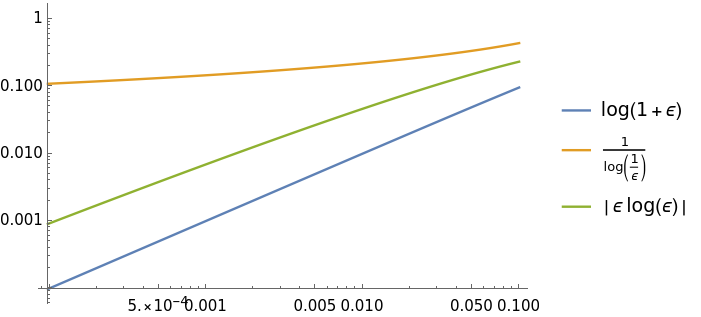
\includegraphics[width = 0.45\textwidth]{Images/6b.png}
		\end{figure}
		
		\newpage
		\item Given
		\begin{gather*}
			\ln(1 + \eps) = O(\eps), \\
			\sech^{-1}\eps = \ln \left(\sqrt{\frac{1}{\eps}-1} \sqrt{\frac{1}{\eps}+1}+\frac{1}{\eps}\right) = O\left(\ln \frac{1}{\eps}\right), \\
			\frac{1 - \cos \eps}{1 + \cos \eps} = O(\eps^2), \\
			\sqrt{\eps(1 - \eps)} = O(\eps^{1/2}), \\
			e^{-\cosh(1/\eps)} = O(e^{-e^{1/\eps}}), \\
			\ln\left(1 + \frac{\ln((1+2\eps)/\eps)}{1-2\eps}\right) = O\left(\ln\left(\ln \frac{1}{\eps}\right)\right), \\
			\ln\left(1 + \frac{\ln(1+\eps)}{\eps(1-2\eps)}\right) = O(1), \\
			\frac{\eps^{1/2}}{1 - \cos \eps} = O(\eps^{-3/2})
		\end{gather*} 
		which can be ordered as
		\begin{align*}
			\frac{\eps^{1/2}}{1 - \cos \eps} &\gg \sech^{-1}\eps \\
			&\gg \ln\left(1 + \frac{\ln((1+2\eps)/\eps)}{1-2\eps}\right) \\
			&\gg \ln\left(1 + \frac{\ln(1+\eps)}{\eps(1-2\eps)}\right) \\
			&\gg \sqrt{\eps(1 - \eps)} \\
			&\gg \ln(1 + \eps) \\
			&\gg \frac{1- \cos \eps}{1 + \cos \eps} \\
			&\gg e^{-\cosh(1 / \eps)}
		\end{align*}
		Again, the complex log terms were the trickiest to place in the list but after a little bit of playing I reduced them down to orders that I could make sense of.
	\end{enumerate}
\end{enumerate}
\end{document}
